\chapter{Evaluation and Testing}\label{testing}

    This chapter presents an evaluation of the application, which is divided into three parts.
    The first part will show variables that must be controlled for the reliability and stability of the result.
    The second part is going to evaluate the application's performance,
    which are comparisons among models, programming languages, and technologies.
    The last section is going to show a usability testing of this application.

    \section{Controlled Variables}
        To ensure the result of the performance will not be varied by other factors, some variables must be controlled as following:
        \begin{enumerate}
            \item All testing cases will be run on Samsung Galaxy S10+.
            \item All running background applications will be closed, and memory will be freed before testing.
            \item To prevent CPU's speed is limited, a power management mode will be set to "Optimised".
            \item Total number of frames in the testing video will be set to 31 frames.
            \item A testing video resolution will be set to 540x480 pixels.
        \end{enumerate}

    \section{Performace Evaluation}
        In this section, the performance of detection models will be compared, and the result will be discussed.
        There are three sections of discussion. The first section will show the result of processing a single frame.
        The second section will compare the performance among a number of threads.
        The last section will discuss the result of NEON instruction and improvement.
        Computation time and frame rate are used as a measurement to o evaluate the performance of the application.
        Frame rate is a number of frames that application can process in 1 second.
        The sample of pre-recorded file is obtained from Ben Benfold and Ian Reid \cite{benfold2009attention}.

        \subsection{Single Frame Comparison}
            In this section, the performance of 2 detection models will be compare, regardless of other tools and techniques.
            To evaluate the performance, each model will process on a single frame.
            There are two different resolutions used as inputs for comparing the performance and understanding the variation of calculation time.

            % Picture Performance Table
            \begin{table}[!htp]\centering
                \scriptsize
                \begin{tabular}{lrrrrrr}\toprule
                    \multicolumn{2}{c}{Model} &\multicolumn{2}{c}{YOLO} &\multicolumn{2}{c}{SSD} \\\midrule
                    \multicolumn{2}{c}{Size} &960×540 &540x480 &960×540 &540x480 \\
                    \multicolumn{2}{c}{Total Process Time (second)} &4.235 &3.827 &0.337 &0.323 \\
                    \multicolumn{2}{c}{Forward Propagation per frame (second)} &3.456 &3.019 &0.284 &0.278 \\
                    \multicolumn{2}{c}{Forward Propagation per frame (perenctage)} &81.61\% &78.89\% &84.27\% &86.07\% \\
                    \bottomrule
                \end{tabular}

                \caption{Picture Processing Performace}\label{performance:picture}
            \end{table}

            As can be seen from table \ref{performance:picture}, the processing time of YOLO model significantly increases when the size of the picture is greater.
            In contrast, MobileNet SSD is able to process the given picture faster than YOLO model \cite{tensorflow2015-whitepaper}, \cite{YOLO-v3}.
            The processing time of MobileNet SSD slightly increases when the size of the picture is increased.

        \subsection{Multithreading}

            % Introduction
            In this section, the performance of both models will be evaluated with multithreading technique,
            and the evaluation will be divided into three parts: sequential computing, YOLO with multithreading, and MobileNet SSD with multithreading.
            As mentions previous section, in this evaluation, controlled variables are set.
            The number of frames in the testing video will be set to 31 frames.

            % Sequential Programming
            For the first part, an application will process the testing video sequentially and measure the performance.
            This measurement will be compared to multithreading and evaluate the improvement of the performance.
            As a result in table \ref{yolo:official-performace} and \ref{ssd:official-performace},
            YOLO model took 102.972 seconds to processed 31 frames video, while MobileNet SSD model took 7.132 seconds.

            % YOLO Model Performace Table
            \begin{table}[!htp]\centering
                \scriptsize
                \begin{tabular}{lrrrrrrr}\toprule
                    \multicolumn{2}{c}{Model} &\multicolumn{5}{c}{YOLO} \\\cmidrule{1-7}
                    \multicolumn{2}{c}{\multirow{2}{*}{}} &\multirow{2}{*}{Sequential Computing} &\multicolumn{4}{c}{Parallel Computing} \\\cmidrule{4-7}
                    & & &1 Thread &2 Threads &4 Threads &8 Threads \\\midrule
                    \multicolumn{2}{c}{Total Process Time (second)} &102.972 &117.805 &96.415 &92.242 &99.441 \\
                    \multicolumn{2}{c}{Garbage Collector (second)} &- &0.102 &0.280 &2.024 &11.333 \\
                    \multicolumn{2}{c}{Process Time without GC} &- &117.703 &96.136 &90.218 &88.108 \\
                    \multicolumn{2}{c}{Forward Propagation (Total)} &79.097 &- &- &- &- \\
                    \multicolumn{2}{c}{Forward Propagation (Average)} &2.553 &2.872 &4.840 &9.231 &19.713 \\
                    \multicolumn{2}{c}{Forward Propagation (Min)} &2.213 &2.564 &4.003 &5.478 &14.733 \\
                    \multicolumn{2}{c}{Forward Propagation (Max)} &2.693 &3.092 &6.436 &12.566 &21.815 \\
                    \multicolumn{2}{c}{Number of frame} &31 &31 &31 &31 &31 \\
                    \multicolumn{2}{c}{Process per frame (second)} &3.322 &3.800 &3.110 &2.976 &3.208 \\
                    \multicolumn{2}{c}{Improvement} & & &18.16\% &21.70\% &15.59\% \\
                    \bottomrule
                \end{tabular}

                \caption{Video Processing with YOLO Model with official build}\label{yolo:official-performace}
            \end{table}

            % Introduction to Multithreading
            Then, a multithreading technique is implemented to increase performance and achieve real-time processing.
            To evaluate the improvement of multithreading, a number of processors will be doubled as follows: 1, 2, 4, and 8.
            In the testing device, there are 8 physical cores, so it can effectively process up to 8 threads.

            % SSD Model Performace Table
            \begin{table}[!htp]\centering
                \scriptsize
                \begin{tabular}{lrrrrrrr}\toprule
                    \multicolumn{2}{c}{Model} &\multicolumn{5}{c}{MobileNet SSD} \\\cmidrule{1-7}
                    \multicolumn{2}{c}{\multirow{2}{*}{}} &\multirow{2}{*}{Sequential Computing} &\multicolumn{4}{c}{Multithreading} \\\cmidrule{4-7}
                    & & &1 Thread &2 Threads &4 Threads &8 Threads \\\midrule
                    \multicolumn{2}{c}{Total Process Time (second)} &7.132 &8.237 &6.873 &6.270 &5.064 \\
                    \multicolumn{2}{c}{Garbage Collector (second)} &- &- &- &- &- \\
                    \multicolumn{2}{c}{Process Time without GC} &- &- &- &- &- \\
                    \multicolumn{2}{c}{Forward Propagation (Total)} &7.019 &- &- &- &- \\
                    \multicolumn{2}{c}{Forward Propagation (Average)} &0.226 &0.235 &0.401 &0.738 &1.133 \\
                    \multicolumn{2}{c}{Forward Propagation (Min)} &0.218 &0.212 &0.353 &0.406 &0.466 \\
                    \multicolumn{2}{c}{Forward Propagation (Max)} &0.243 &0.320 &0.456 &1.477 &2.582 \\
                    \multicolumn{2}{c}{Number of frame} &31 &31 &31 &31 &31 \\
                    \multicolumn{2}{c}{Process per frame (second)} &0.230 &0.266 &0.222 &0.202 &0.163 \\
                    \multicolumn{2}{c}{Improvement} & & &16.56\% &23.88\% &38.52\% \\
                    \bottomrule
                \end{tabular}

                \caption{MobileNet SSD Model with OpenCV official build in Java}\label{ssd:official-performace}
            \end{table}

            % YOLO with multithreading
            As shown in table \ref{yolo:official-performace},
                the performance of 2 threads is improved only 18.16 per cent,
                and it reaches the best performance at 21.7 per cent by using 4 threads.
            However, the performance of 8 threads is worse than 2 threads.
                One of the factors is the Garbage Collection (GC).
                The application was frozen while GC is collecting garbage.
            GC is not collecting only short-lived objects but long-lived objects as well,
                and GC is more often collect garbage when the number of threads is increased.

            As shown in figure \ref{yolo:memoryUsage}, memory was allocated by double and array of double,
                and GC was freeing these allocation 10 times within 5 seconds.
            Consequently, CPU usage is dropped when GC is working.
                This problem can be seen in figure \ref{yolo:cpuUsage}.
                The progress status will be green when a thread is working.
                It will be yellow when a thread is interrupted by GC,
                and it will be grey when a thread has no activity.

            % CPU Usage
            \begin{figure}[!ht]
                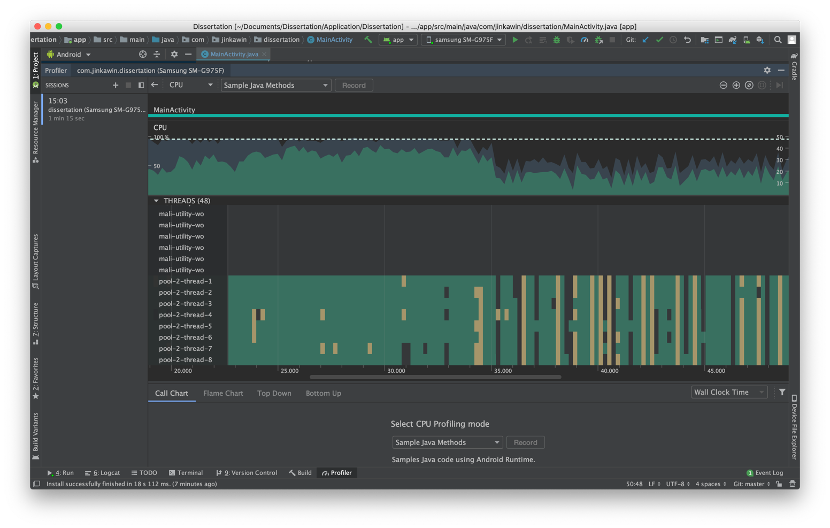
\includegraphics[width=6in]{images/chapter5/YOLO/cpu-usage-8threads.png}
                \caption{CPU Usage of YOLO Model with 8 threads}
                \label{yolo:cpuUsage}
            \end{figure}

            % Memory Usgae
            \begin{figure}[!ht]
                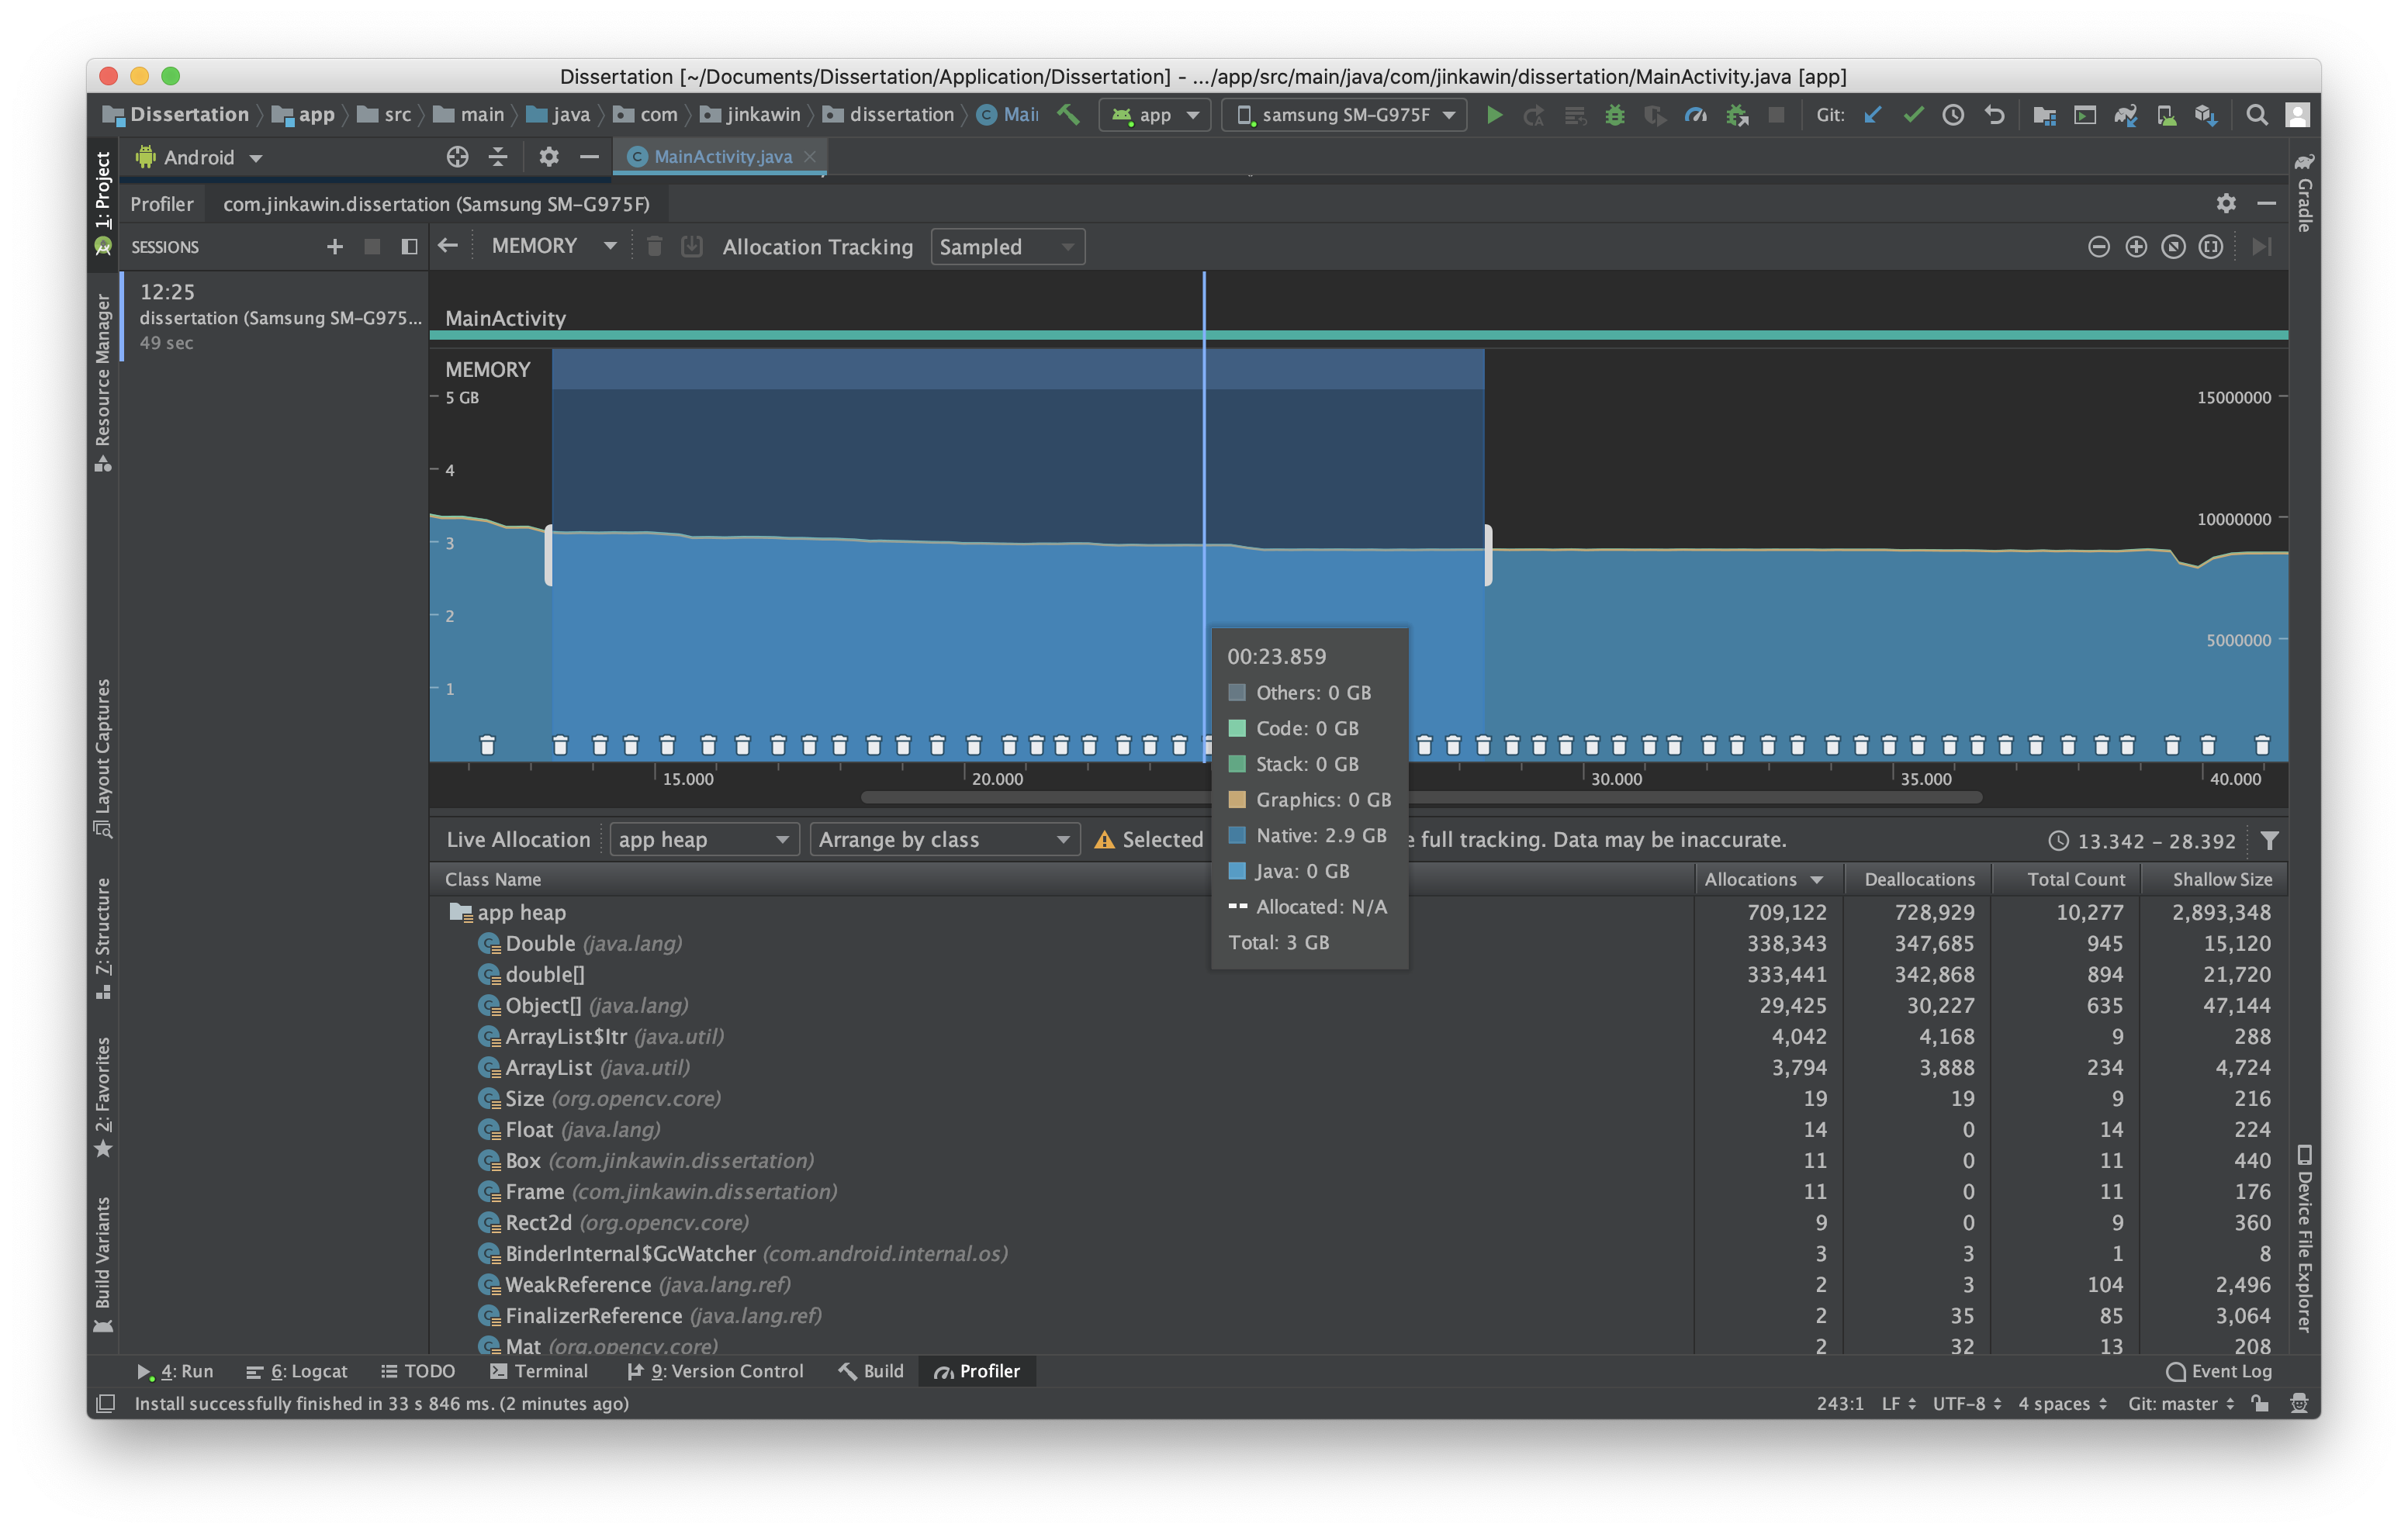
\includegraphics[width=6in]{images/chapter5/gc-problem/gc-collecting.png}
                \caption{Memory Usage of YOLO Model with 8 threads}
                \label{yolo:memoryUsage}
            \end{figure}

            % SSD with multithreading
            For the MobileNet SSD model,
            the calculation time of 2 threads is improved only 16.56 per cent,
            and 8 threads give the best performance with 38.53 per cent as can be seen in table \ref{ssd:official-performace}.
            Objects are not collected by GC in this model, but memory will be freed after processing is finished.
            The improvement computation time of 8 threads by using MobileNet SSD model is better than YOLO model,
            but the speed-up time of both models still lower than an ideal time.

            % Conclusion and tasking about recompile model and NEON
            In summary, the overall performance of YOLO model with multithreading is slightly improved,
            and it becomes worse when using 8 threads.
            Regarding this examination, one of the obvious factors of these problems is
            GC.
            In contrast, the speed-up scale of MobileNet SSD is better than YOLO model because there is no
            GC during processing.
            YOLO model uses more memory than MobileNet SSD in term of variables in double type.

        \subsection{Android Native Development Kit}

            \begin{table}[!htp]\centering
                \scriptsize
                \begin{tabular}{lrrrrrrr}\toprule
                    \multicolumn{2}{c}{Model} &\multicolumn{5}{c}{MobileNet SSD} \\\cmidrule{1-7}
                    \multicolumn{2}{c}{\multirow{2}{*}{}} &\multirow{2}{*}{Sequential Computing} &\multicolumn{4}{c}{Multithreading} \\\cmidrule{4-7}
                    & & &1 Thread &2 Threads &4 Threads &8 Threads \\\midrule
                    \multicolumn{2}{c}{Total Process Time (second)} &6.773 &11.949 &6.597 &6.150 &4.954 \\
                    \multicolumn{2}{c}{Garbage Collector (second)} &- &- &- &- &- \\
                    \multicolumn{2}{c}{Process Time without GC} &- &- &- &- &- \\
                    \multicolumn{2}{c}{Forward Propagation (Total)} &6.659 &- &- &- &- \\
                    \multicolumn{2}{c}{Forward Propagation (Average)} &0.215 &0.382 &0.408 &0.613 &0.970 \\
                    \multicolumn{2}{c}{Forward Propagation (Min)} &0.198 &0.363 &0.394 &0.405 &0.407 \\
                    \multicolumn{2}{c}{Forward Propagation (Max)} &0.236 &0.401 &0.421 &1.043 &2.691 \\
                    \multicolumn{2}{c}{Number of frame} &31 &31 &31 &31 &31 \\
                    \multicolumn{2}{c}{Process per frame (second)} &0.218 &0.385 &0.213 &0.198 &0.160 \\
                    \multicolumn{2}{c}{Improvement} & & &44.79\% &48.53\% &58.54\% \\
                    \bottomrule
                \end{tabular}

                \caption{MobileNet SSD Model with OpenCV official build in C++}\label{ssd:official-performace-cpp}
            \end{table}

            As mentioned in the chapter \ref{implement},
            detection process and distance measurement can be written in C++ to achieve higher performance.
            As it can be seen in table \ref{ssd:official-performace-cpp},
            the performance of using 2 threads is improved 44.79 per cent when compared to using 1 thread,
            and the performance is fastened up to 58.54 per cent when using 8 threads.
            However, there are 2 issues of this implementation.
            The first issues is the forward propagation time.
                Theoretically, the processing time of sequential computing and using a single thread should be the same.
                In contrast, the forward propagation time of single thread was doubled,
                which causes total process time increase.
                Due to the thread management system in C++ is different when compared to Java.
                In C++, the thread is managed by OpenCV's parallelism framework, while
                the thread pool is used in Java which is recommended by Android's document \cite{ANDROID-01}, \cite{opencv_library}.
            The second issue is the total process time.
                Although writing in C++ is able to achieve theoretical speed-up,
                the overall performance is slightly better when compared to Java.

        \subsection{NEON Instruction}
            OpenCV library provides a shared library, which is officially built by OpenCV.
            However, the library is built to support all CPU chipsets, and many features and conditions were flagged during building.
            The library is needed to be manually built from scratch to evaluate the performance of NEON \cite{NEON-ARM}.
            OpenCV shared library was manually built into two versions: version with NEON and version without NEON.
            To maximise the performance of the NEON version, OpenCV is forced to be built with NEON instruction regardless of any condition,
            and it will support only ARMv8-A 64-bit architecture.

            \begin{table}[!htp]\centering
                \scriptsize
                \begin{tabular}{lrrrrrrr}\toprule
                    \multicolumn{2}{c}{Model} &\multicolumn{5}{c}{MobileNet SSD without NEON} \\\cmidrule{1-7}
                    \multicolumn{2}{c}{\multirow{2}{*}{}} &\multirow{2}{*}{Sequential Computing} &\multicolumn{4}{c}{Parallel Computing} \\\cmidrule{4-7}
                    & & &1 Thread &2 Threads &4 Threads &8 Threads \\\midrule
                    \multicolumn{2}{c}{Total Process Time (second)} &17.308 &19.030 &15.172 &11.797 &10.624 \\
                    \multicolumn{2}{c}{Garbage Collector (second)} &- &- &- &- &- \\
                    \multicolumn{2}{c}{Process Time without GC} &- &- &- &- &- \\
                    \multicolumn{2}{c}{Forward Propagation (Total)} &17.193 &17.848 &- &- &- \\
                    \multicolumn{2}{c}{Forward Propagation (Average)} &0.555 &0.576 &0.926 &1.416 &2.462 \\
                    \multicolumn{2}{c}{Forward Propagation (Min)} &0.519 &0.545 &0.582 &0.756 &1.310 \\
                    \multicolumn{2}{c}{Forward Propagation (Max)} &0.586 &0.654 &1.412 &2.593 &5.308 \\
                    \multicolumn{2}{c}{Number of frame} &31 &31 &31 &31 &31 \\
                    \multicolumn{2}{c}{Process per frame (second)} &0.558 &0.614 &0.489 &0.381 &0.343 \\
                    \multicolumn{2}{c}{Improvement} & & &20.27\% &38.01\% &44.17\% \\
                    \bottomrule
                \end{tabular}

                \caption{MobileNet SSD Model with OpenCV manully build ({\bf without} NEON)}\label{ssd:non-neon-performance}
            \end{table}

            \begin{table}[!htp]\centering
                \scriptsize
                \begin{tabular}{lrrrrrrr}\toprule
                    \multicolumn{2}{c}{Model} &\multicolumn{5}{c}{MobileNet SSD with NEON} \\\cmidrule{1-7}
                    \multicolumn{2}{c}{\multirow{2}{*}{}} &\multirow{2}{*}{Sequential Computing} &\multicolumn{4}{c}{Multithreading} \\\cmidrule{4-7}
                    & & &1 Thread &2 Threads &4 Threads &8 Threads \\\midrule
                    \multicolumn{2}{c}{Total Process Time (second)} &4.006 &6.079 &4.208 &3.127 &2.890 \\
                    \multicolumn{2}{c}{Garbage Collector (second)} &- &- &- &- &- \\
                    \multicolumn{2}{c}{Process Time without GC} &- &- &- &- &- \\
                    \multicolumn{2}{c}{Forward Propagation (Total)} &3.927 &4.950 &- &- &- \\
                    \multicolumn{2}{c}{Forward Propagation (Average)} &0.126 &0.159 &0.225 &0.339 &0.645 \\
                    \multicolumn{2}{c}{Forward Propagation (Min)} &0.117 &0.128 &0.131 &0.190 &0.266 \\
                    \multicolumn{2}{c}{Forward Propagation (Max)} &0.135 &0.250 &0.295 &0.596 &1.798 \\
                    \multicolumn{2}{c}{Number of frame} &31 &31 &31 &31 &31 \\
                    \multicolumn{2}{c}{Process per frame (second)} &0.129 &0.196 &0.136 &0.101 &0.093 \\
                    \multicolumn{2}{c}{Improvement} & & &30.78\% &48.56\% &52.46\% \\
                    \bottomrule
                \end{tabular}

                \caption{Video Processing with MobileNet SSD Model ({\bf with} NEON)}\label{ssd:neon-performance}
            \end{table}

            After OpenCV library is manually built and forced to be compiled with NEON instruction,
            the performance of human detection is significantly improved.
            As can be seen in table \ref{ssd:non-neon-performance} and \ref{ssd:neon-performance},
            the sequential computing took 4 second for processing human detection,
            which is faster than OpenCV without NEON 76.85 percent.
            In addition, multithreading can process 31 frames of the video up to 2.890 seconds,
            which is faster than OpenCV without NEON 72.79 per cent and OpenCV official build 42.93 per cent.
            For this performance, video can be processed 10.75 frames per second.
            In addition, according to rendering technique in chapter \ref{implement},
            a real-time video from the camera can display up to 25 frames per second.

    % Analyse
    Thus far, these results were not achieved theoretical,
    and this application did not achieve processing and displaying 30 FPS even if
    multithreading and NEON are implemented.
    This underachieved performance could be caused by mulithreading itself.
    A forward propagation time, which took most of the computation time, is doubled when the number of threads is increased.
        One of the issues that emerge from this finding is parallelisation in the OpenCV library.
        Some function underneath the forward propagation function is parallelised by using multithreading.
        Then, when a frame processing thread is created, a number of threads may exceed the number of physical cores.
        Thus, threads are interrupted, and it caused a context switching overhead.
    Besides, the calculation time of using a single thread is always greater than
    the calculation time un sequential computing and it could be caused by this problem.